% -*- Mode:TeX -*-

%% IMPORTANT: The official thesis specifications are available at:
%%            http://libraries.mit.edu/archives/thesis-specs/
%%
%%            Please verify your thesis' formatting and copyright
%%            assignment before submission.  If you notice any
%%            discrepancies between these templates and the 
%%            MIT Libraries' specs, please let us know
%%            by e-mailing thesis@mit.edu

%% The documentclass options along with the pagestyle can be used to generate
%% a technical report, a draft copy, or a regular thesis.  You may need to
%% re-specify the pagestyle after you \include  cover.tex.  For more
%% information, see the first few lines of mitthesis.cls. 

%\documentclass[12pt,vi,twoside]{mitthesis}
%%
%%  If you want your thesis copyright to you instead of MIT, use the
%%  ``vi'' option, as above.
%%
%\documentclass[12pt,twoside,leftblank]{mitthesis}
%%
%% If you want blank pages before new chapters to be labelled ``This
%% Page Intentionally Left Blank'', use the ``leftblank'' option, as
%% above. 

\documentclass[12pt]{mitthesis}
\usepackage{lgrind}
%% These have been added at the request of the MIT Libraries, because
%% some PDF conversions mess up the ligatures.  -LB, 1/22/2014
\usepackage{cmap}
\usepackage[T1]{fontenc}
\pagestyle{plain}

%% This bit allows you to either specify only the files which you wish to
%% process, or `all' to process all files which you \include.
%% Krishna Sethuraman (1990).

\def\files{cover,contents,chap1}
\def\all{all}
\includeonly{\files} 

\begin{document}

% -*-latex-*-
% 
% For questions, comments, concerns or complaints:
% thesis@mit.edu
% 
%
% $Log: cover.tex,v $
% Revision 1.8  2008/05/13 15:02:15  jdreed
% Degree month is June, not May.  Added note about prevdegrees.
% Arthur Smith's title updated
%
% Revision 1.7  2001/02/08 18:53:16  boojum
% changed some \newpages to \cleardoublepages
%
% Revision 1.6  1999/10/21 14:49:31  boojum
% changed comment referring to documentstyle
%
% Revision 1.5  1999/10/21 14:39:04  boojum
% *** empty log message ***
%
% Revision 1.4  1997/04/18  17:54:10  othomas
% added page numbers on abstract and cover, and made 1 abstract
% page the default rather than 2.  (anne hunter tells me this
% is the new institute standard.)
%
% Revision 1.4  1997/04/18  17:54:10  othomas
% added page numbers on abstract and cover, and made 1 abstract
% page the default rather than 2.  (anne hunter tells me this
% is the new institute standard.)
%
% Revision 1.3  93/05/17  17:06:29  starflt
% Added acknowledgements section (suggested by tompalka)
% 
% Revision 1.2  92/04/22  13:13:13  epeisach
% Fixes for 1991 course 6 requirements
% Phrase "and to grant others the right to do so" has been added to 
% permission clause
% Second copy of abstract is not counted as separate pages so numbering works
% out
% 
% Revision 1.1  92/04/22  13:08:20  epeisach

% NOTE:
% These templates make an effort to conform to the MIT Thesis specifications,
% however the specifications can change.  We recommend that you verify the
% layout of your title page with your thesis advisor and/or the MIT 
% Libraries before printing your final copy.
\title{An Optimizing Compiler for Low-Level Floating Point Operations}

\author{Eric Lubin}
% If you wish to list your previous degrees on the cover page, use the 
% previous degrees command:
%       \prevdegrees{A.A., Harvard University (1985)}
% You can use the \\ command to list multiple previous degrees
%       \prevdegrees{B.S., University of California (1978) \\
%                    S.M., Massachusetts Institute of Technology (1981)}
\department{Department of Electrical Engineering and Computer Science}

% If the thesis is for two degrees simultaneously, list them both
% separated by \and like this:
% \degree{Doctor of Philosophy \and Master of Science}
\degree{Bachelor of Science in Computer Science and Engineering}

% As of the 2007-08 academic year, valid degree months are September, 
% February, or June.  The default is June.
\degreemonth{February}
\degreeyear{2015}
\thesisdate{January 1, 2015}

%% By default, the thesis will be copyrighted to MIT.  If you need to copyright
%% the thesis to yourself, just specify the `vi' documentclass option.  If for
%% some reason you want to exactly specify the copyright notice text, you can
%% use the \copyrightnoticetext command.  
%\copyrightnoticetext{\copyright IBM, 1990.  Do not open till Xmas.}

% If there is more than one supervisor, use the \supervisor command
% once for each.
\supervisor{Jim Yang}{Sr. Manager, R\&D, VMware}
\supervisor{Martin C. Rinard}{Professor}
% This is the department committee chairman, not the thesis committee
% chairman.  You should replace this with your Department's Committee
% Chairman.
\chairman{Dennis M. Freeman}{Chairman, Department Committee on Graduate Theses}

% Make the titlepage based on the above information.  If you need
% something special and can't use the standard form, you can specify
% the exact text of the titlepage yourself.  Put it in a titlepage
% environment and leave blank lines where you want vertical space.
% The spaces will be adjusted to fill the entire page.  The dotted
% lines for the signatures are made with the \signature command.
\maketitle

% The abstractpage environment sets up everything on the page except
% the text itself.  The title and other header material are put at the
% top of the page, and the supervisors are listed at the bottom.  A
% new page is begun both before and after.  Of course, an abstract may
% be more than one page itself.  If you need more control over the
% format of the page, you can use the abstract environment, which puts
% the word "Abstract" at the beginning and single spaces its text.

%% You can either \input (*not* \include) your abstract file, or you can put
%% the text of the abstract directly between the \begin{abstractpage} and
%% \end{abstractpage} commands.

% First copy: start a new page, and save the page number.
\cleardoublepage
% Uncomment the next line if you do NOT want a page number on your
% abstract and acknowledgments pages.
% \pagestyle{empty}
\setcounter{savepage}{\thepage}
\begin{abstractpage}
% $Log: abstract.tex,v $
% Revision 1.1  93/05/14  14:56:25  starflt
% Initial revision
% 
% Revision 1.1  90/05/04  10:41:01  lwvanels
% Initial revision
% 
%
%% The text of your abstract and nothing else (other than comments) goes here.
%% It will be single-spaced and the rest of the text that is supposed to go on
%% the abstract page will be generated by the abstractpage environment.  This
%% file should be \input (not \include 'd) from cover.tex.
In this thesis, I designed and implemented a compiler which performs
optimizations that reduce the number of low-level floating point operations
necessary for a specific task; this involves the optimization of chains of
floating point operations as well as the implementation of a ``fixed'' point
data type that allows some floating point operations to simulated with integer
arithmetic.  The source language of the compiler is a subset of C, and the
destination language is assembly language for a micro-floating point CPU.  An
instruction-level simulator of the CPU was written to allow testing of the
code.  A series of test pieces of codes was compiled, both with and without
optimization, to determine how effective these optimizations were.

\end{abstractpage}

% Additional copy: start a new page, and reset the page number.  This way,
% the second copy of the abstract is not counted as separate pages.
% Uncomment the next 6 lines if you need two copies of the abstract
% page.
% \setcounter{page}{\thesavepage}
% \begin{abstractpage}
% % $Log: abstract.tex,v $
% Revision 1.1  93/05/14  14:56:25  starflt
% Initial revision
% 
% Revision 1.1  90/05/04  10:41:01  lwvanels
% Initial revision
% 
%
%% The text of your abstract and nothing else (other than comments) goes here.
%% It will be single-spaced and the rest of the text that is supposed to go on
%% the abstract page will be generated by the abstractpage environment.  This
%% file should be \input (not \include 'd) from cover.tex.
In this thesis, I designed and implemented a compiler which performs
optimizations that reduce the number of low-level floating point operations
necessary for a specific task; this involves the optimization of chains of
floating point operations as well as the implementation of a ``fixed'' point
data type that allows some floating point operations to simulated with integer
arithmetic.  The source language of the compiler is a subset of C, and the
destination language is assembly language for a micro-floating point CPU.  An
instruction-level simulator of the CPU was written to allow testing of the
code.  A series of test pieces of codes was compiled, both with and without
optimization, to determine how effective these optimizations were.

% \end{abstractpage}

\cleardoublepage

\section*{Acknowledgments}

This is the acknowledgements section.  You should replace this with your
own acknowledgements.

%%%%%%%%%%%%%%%%%%%%%%%%%%%%%%%%%%%%%%%%%%%%%%%%%%%%%%%%%%%%%%%%%%%%%%
% -*-latex-*-

% Some departments (e.g. 5) require an additional signature page.  See
% signature.tex for more information and uncomment the following line if
% applicable.
% % -*- Mode:TeX -*-
%
% Some departments (e.g. Chemistry) require an additional cover page
% with signatures of the thesis committee.  Please check with your
% thesis advisor or other appropriate person to determine if such a 
% page is required for your thesis.  
%
% If you choose not to use the "titlepage" environment, a \newpage
% commands, and several \vspace{\fill} commands may be necessary to
% achieve the required spacing.  The \signature command is defined in
% the "mitthesis" class
%
% The following sample appears courtesy of Ben Kaduk <kaduk@mit.edu> and
% was used in his June 2012 doctoral thesis in Chemistry. 

\begin{titlepage}
\begin{large}
This doctoral thesis has been examined by a Committee of the Department
of Chemistry as follows:

\signature{Professor Jianshu Cao}{Chairman, Thesis Committee \\
   Professor of Chemistry}

\signature{Professor Troy Van Voorhis}{Thesis Supervisor \\
   Associate Professor of Chemistry}

\signature{Professor Robert W. Field}{Member, Thesis Committee \\
   Haslam and Dewey Professor of Chemistry}
\end{large}
\end{titlepage}


\pagestyle{plain}
  % -*- Mode:TeX -*-
%% This file simply contains the commands that actually generate the table of
%% contents and lists of figures and tables.  You can omit any or all of
%% these files by simply taking out the appropriate command.  For more
%% information on these files, see appendix C.3.3 of the LaTeX manual. 
\tableofcontents
\newpage
\listoffigures
\newpage
\listoftables


%% This is an example first chapter.  You should put chapter/appendix that you
%% write into a separate file, and add a line \include{yourfilename} to
%% main.tex, where `yourfilename.tex' is the name of the chapter/appendix file.
%% You can process specific files by typing their names in at the 
%% \files=
%% prompt when you run the file main.tex through LaTeX.
\chapter{Introduction}


Micro-optimization is a technique to reduce the overall operation count of
floating point operations.  In a standard floating point unit, floating
point operations are fairly high level, such as ``multiply'' and ``add'';
in a micro floating point unit ($\mu$FPU), these have been broken down into
their constituent low-level floating point operations on the mantissas and
exponents of the floating point numbers.

Chapter two describes the architecture of the $\mu$FPU unit, and the
motivations for the design decisions made.

Chapter three describes the design of the compiler, as well as how the
optimizations discussed in section~\ref{ch1:opts} were implemented.

Chapter four describes the purpose of test code that was compiled, and which
statistics were gathered by running it through the simulator.  The purpose
is to measure what effect the micro-optimizations had, compared to
unoptimized code.  Possible future expansions to the project are also
discussed.

\section{Motivations for micro-optimization}

The idea of micro-optimization is motivated by the recent trends in computer
architecture towards low-level parallelism and small, pipelineable
instruction sets \cite{patterson:risc,rad83}.  By getting rid of more
complex instructions and concentrating on optimizing frequently used
instructions, substantial increases in performance were realized.

Another important motivation was the trend towards placing more of the
burden of performance on the compiler.  Many of the new architectures depend
on an intelligent, optimizing compiler in order to realize anywhere near
their peak performance
\cite{ellis:bulldog,pet87,coutant:precision-compilers}.  In these cases, the
compiler not only is responsible for faithfully generating native code to
match the source language, but also must be aware of instruction latencies,
delayed branches, pipeline stages, and a multitude of other factors in order
to generate fast code \cite{gib86}.

Taking these ideas one step further, it seems that the floating point
operations that are normally single, large instructions can be further broken
down into smaller, simpler, faster instructions, with more control in the
compiler and less in the hardware.  This is the idea behind a
micro-optimizing FPU; break the floating point instructions down into their
basic components and use a small, fast implementation, with a large part of
the burden of hardware allocation and optimization shifted towards
compile-time.

Along with the hardware speedups possible by using a $\mu$FPU, there are
also optimizations that the compiler can perform on the code that is
generated.  In a normal sequence of floating point operations, there are
many hidden redundancies that can be eliminated by allowing the compiler to
control the floating point operations down to their lowest level.  These
optimizations are described in detail in section~\ref{ch1:opts}.

\section{Description of micro-optimization}\label{ch1:opts}

In order to perform a sequence of floating point operations, a normal FPU
performs many redundant internal shifts and normalizations in the process of
performing a sequence of operations.  However, if a compiler can
decompose the floating point operations it needs down to the lowest level,
it then can optimize away many of these redundant operations.  

If there is some additional hardware support specifically for
micro-optimization, there are additional optimizations that can be
performed.  This hardware support entails extra ``guard bits'' on the
standard floating point formats, to allow several unnormalized operations to
be performed in a row without the loss information\footnote{A description of
the floating point format used is shown in figures~\ref{exponent-format}
and~\ref{mantissa-format}.}.  A discussion of the mathematics behind
unnormalized arithmetic is in appendix~\ref{unnorm-math}.

The optimizations that the compiler can perform fall into several categories:

\subsection{Post Multiply Normalization}

When more than two multiplications are performed in a row, the intermediate
normalization of the results between multiplications can be eliminated.
This is because with each multiplication, the mantissa can become
denormalized by at most one bit.  If there are guard bits on the mantissas
to prevent bits from ``falling off'' the end during multiplications, the
normalization can be postponed until after a sequence of several
multiplies\footnote{Using unnormalized numbers for math is not a new idea; a
good example of it is the Control Data CDC 6600, designed by Seymour Cray.
\cite{thornton:cdc6600} The CDC 6600 had all of its instructions performing
unnormalized arithmetic, with a separate {\tt NORMALIZE} instruction.}.

% This is an example of how you would use tgrind to include an example
% of source code; it is commented out in this template since the code
% example file does not exist.  To use it, you need to remove the '%' on the
% beginning of the line, and insert your own information in the call.
%
%\tagrind[htbp]{code/pmn.s.tex}{Post Multiply Normalization}{opt:pmn}

As you can see, the intermediate results can be multiplied together, with no
need for intermediate normalizations due to the guard bit.  It is only at
the end of the operation that the normalization must be performed, in order
to get it into a format suitable for storing in memory\footnote{Note that
for purposed of clarity, the pipeline delays were considered to be 0, and
the branches were not delayed.}.

\subsection{Block Exponent}

In a unoptimized sequence of additions, the sequence of operations is as
follows for each pair of numbers ($m_1$,$e_1$) and ($m_2$,$e_2$).
\begin{enumerate}
  \item Compare $e_1$ and $e_2$.
  \item Shift the mantissa associated with the smaller exponent $|e_1-e_2|$
        places to the right.
  \item Add $m_1$ and $m_2$.
  \item Find the first one in the resulting mantissa.
  \item Shift the resulting mantissa so that normalized
  \item Adjust the exponent accordingly.
\end{enumerate}

Out of 6 steps, only one is the actual addition, and the rest are involved
in aligning the mantissas prior to the add, and then normalizing the result
afterward.  In the block exponent optimization, the largest mantissa is
found to start with, and all the mantissa's shifted before any additions
take place.  Once the mantissas have been shifted, the additions can take
place one after another\footnote{This requires that for n consecutive
additions, there are $\log_{2}n$ high guard bits to prevent overflow.  In
the $\mu$FPU, there are 3 guard bits, making up to 8 consecutive additions
possible.}.  An example of the Block Exponent optimization on the expression
X = A + B + C is given in figure~\ref{opt:be}.

% This is an example of how you would use tgrind to include an example
% of source code; it is commented out in this template since the code
% example file does not exist.  To use it, you need to remove the '%' on the
% beginning of the line, and insert your own information in the call.
%
%\tgrind[htbp]{code/be.s.tex}{Block Exponent}{opt:be}

\section{Integer optimizations}

As well as the floating point optimizations described above, there are
also integer optimizations that can be used in the $\mu$FPU.  In concert
with the floating point optimizations, these can provide a significant
speedup.  

\subsection{Conversion to fixed point}

Integer operations are much faster than floating point operations; if it is
possible to replace floating point operations with fixed point operations,
this would provide a significant increase in speed.

This conversion can either take place automatically or or based on a
specific request from the programmer.  To do this automatically, the
compiler must either be very smart, or play fast and loose with the accuracy
and precision of the programmer's variables.  To be ``smart'', the computer
must track the ranges of all the floating point variables through the
program, and then see if there are any potential candidates for conversion
to floating point.  This technique is discussed further in
section~\ref{range-tracking}, where it was implemented.

The other way to do this is to rely on specific hints from the programmer
that a certain value will only assume a specific range, and that only a
specific precision is desired.  This is somewhat more taxing on the
programmer, in that he has to know the ranges that his values will take at
declaration time (something normally abstracted away), but it does provide
the opportunity for fine-tuning already working code.

Potential applications of this would be simulation programs, where the
variable represents some physical quantity; the constraints of the physical
system may provide bounds on the range the variable can take.
\subsection{Small Constant Multiplications}

One other class of optimizations that can be done is to replace
multiplications by small integer constants into some combination of
additions and shifts.  Addition and shifting can be significantly faster
than multiplication.  This is done by using some combination of
\begin{eqnarray*}
a_i & = & a_j + a_k \\
a_i & = & 2a_j + a_k \\
a_i & = & 4a_j + a_k \\
a_i & = & 8a_j + a_k \\
a_i & = & a_j - a_k \\
a_i & = & a_j \ll m \mbox{shift}
\end{eqnarray*}
instead of the multiplication.  For example, to multiply $s$ by 10 and store
the result in $r$, you could use:
\begin{eqnarray*}
r & = & 4s + s\\
r & = & r + r
\end{eqnarray*}
Or by 59:
\begin{eqnarray*}
t & = & 2s + s \\
r & = & 2t + s \\
r & = & 8r + t
\end{eqnarray*}
Similar combinations can be found for almost all of the smaller
integers\footnote{This optimization is only an ``optimization'', of course,
when the amount of time spent on the shifts and adds is less than the time
that would be spent doing the multiplication.  Since the time costs of these
operations are known to the compiler in order for it to do scheduling, it is
easy for the compiler to determine when this optimization is worth using.}.
\cite{magenheimer:precision}

\section{Other optimizations}

\subsection{Low-level parallelism}

The current trend is towards duplicating hardware at the lowest level to
provide parallelism\footnote{This can been seen in the i860; floating point
additions and multiplications can proceed at the same time, and the RISC
core be moving data in and out of the floating point registers and providing
flow control at the same time the floating point units are active. \cite{byte:i860}}

Conceptually, it is easy to take advantage to low-level parallelism in the
instruction stream by simply adding more functional units to the $\mu$FPU,
widening the instruction word to control them, and then scheduling as many
operations to take place at one time as possible.

However, simply adding more functional units can only be done so many times;
there is only a limited amount of parallelism directly available in the
instruction stream, and without it, much of the extra resources will go to
waste.  One process used to make more instructions potentially schedulable
at any given time is ``trace scheduling''.  This technique originated in the
Bulldog compiler for the original VLIW machine, the ELI-512.
\cite{ellis:bulldog,colwell:vliw}  In trace scheduling, code can be
scheduled through many basic blocks at one time, following a single
potential ``trace'' of program execution.  In this way, instructions that
{\em might\/} be executed depending on a conditional branch further down in
the instruction stream are scheduled, allowing an increase in the potential
parallelism.  To account for the cases where the expected branch wasn't
taken, correction code is inserted after the branches to undo the effects of
any prematurely executed instructions.

\subsection{Pipeline optimizations}

In addition to having operations going on in parallel across functional
units, it is also typical to have several operations in various stages of
completion in each unit.  This pipelining allows the throughput of the
functional units to be increased, with no increase in latency.

There are several ways pipelined operations can be optimized.  On the
hardware side, support can be added to allow data to be recirculated back
into the beginning of the pipeline from the end, saving a trip through the
registers.  On the software side, the compiler can utilize several tricks to
try to fill up as many of the pipeline delay slots as possible, as
seendescribed by Gibbons. \cite{gib86}



%% This is an example first chapter.  You should put chapter/appendix that you
%% write into a separate file, and add a line \include{yourfilename} to
%% main.tex, where `yourfilename.tex' is the name of the chapter/appendix file.
%% You can process specific files by typing their names in at the 
%% \files=
%% prompt when you run the file main.tex through LaTeX.
\chapter{Docker Fundamentals}
\label{chap:docker}

Docker is a relatively new open-source framework that serves as a lightweight alternative to virtual machines. It provides users with the ability to create isolated, high-performing containers that can be seamlessly deployed to other hosts that are also running the Docker Engine. Unlike virtual machines, containers share the kernel with the host and therefore rely on specific features in the kernel to provide a comparable level of isolation. For now, these containers are restricted to Linux; however, Microsoft has recently made a commitment to bring container technology based on Docker to the Windows platform \cite{windows-docker}.

For the past few years, Docker has been under active heavy development and in recent months is gaining popularity across the industry. An extraordinary number of new projects and platforms are being built on top of Docker, resulting in a rich and lively ecosystem. 


In section~\ref{ch2:system}, we outline the technical details of Docker; in section~\ref{ch2:lingo}, we describe fundamental terms that will be essential to the understanding of VM2Docker; in section~\ref{ch2:usecase} we dive into the wide variety of use cases Docker containers can have; and finally in section~\ref{ch2:industry} we discuss the industry's response to Docker.

\section{System Details}\label{ch2:system}
The Docker platform is divided into the Docker Engine, which supports the runtime and execution of containers, and the Docker Registry, which provides the hosting and delivery of a repository of Docker images. Each container provides a namespaced, isolated environment for execution. Docker exploits filesystem layering, as well as specific features of the Linux kernel to make all of these possible.

\begin{figure}[h]
\centering
    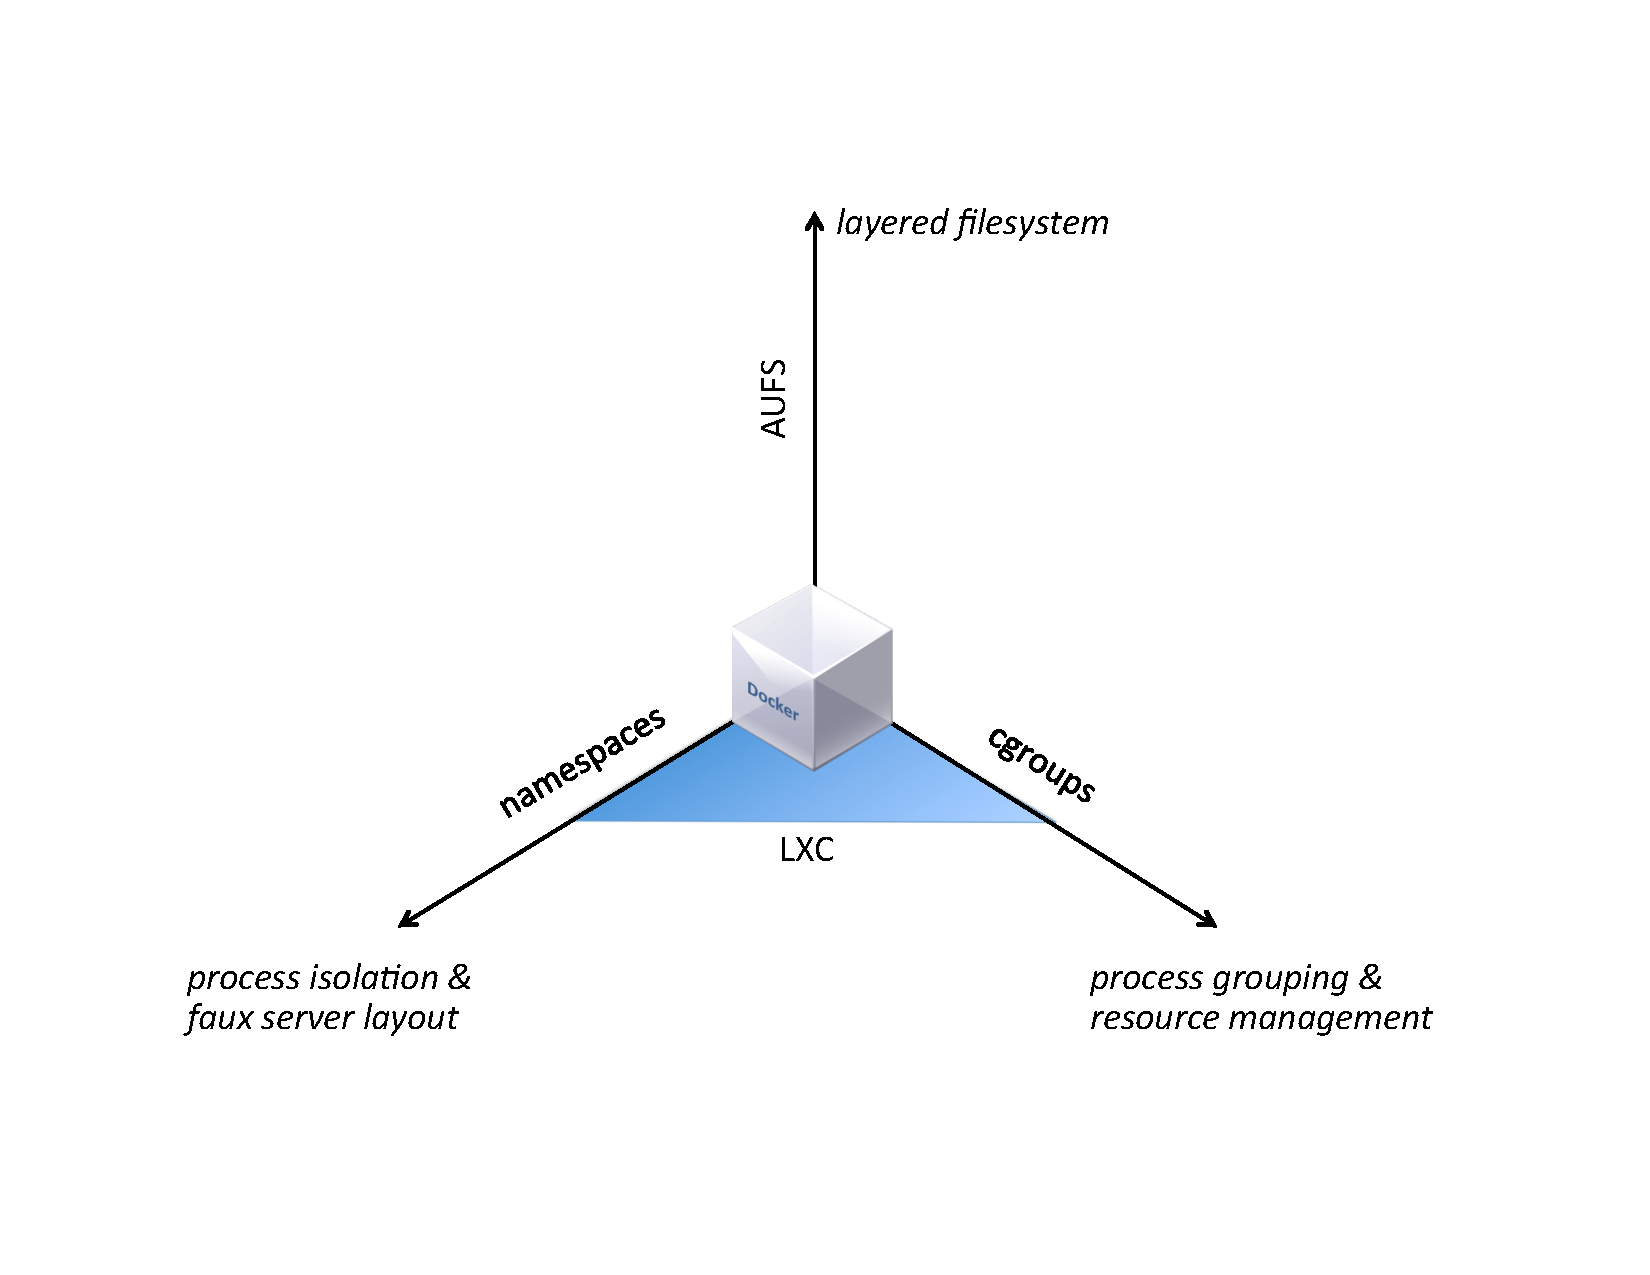
\includegraphics[width=1.0\textwidth]{docker.pdf}
    \caption{A graphic outlining the three fundamental components that make up the Docker framework. Namespace and cgroup support are provided by the LXC (LinuX Container) kernel extensions, and filesystem layering is provided by AUFS.}
\end{figure}

\subsection{cgroups}
Cgroups, or control groups, are a feature on the Linux kernel that provides resource limiting, in the form of memory or disk limits, as well as prioritization of CPU and disk throughput. These features are comparable to those offered by a virtual machine hypervisor to allocate a given amount of memory and CPU, network, and disk priority to a virtual machine.

\subsection{namespaces}

Namespaces are the mechanism by which each Docker container is isolated from the host and other containers. There are many different namespaces that LXC supports, but probably the two most significant ones are the \texttt{pid} and \texttt{net} namespaces. The \texttt{pid} namespace is responsible for giving each container its own isolated environment for processes. A given container can only see and send signals to the processes that are running within the same container. In addition, the \texttt{net} namespace allows different containers to have what appears to be distinct network interfaces, thereby permitting two containers to simultaneously bind to the same port, for example \cite{lxc}.

\subsection{Another Union FileSystem (AUFS)}
AUFS, Another Union FileSystem, is the primary means through which Docker achieves both storage savings and faster deployments of containers. Each image inherits from a sequence of other images, up to the base image, and represents the set or sequence of changes on the filesystem. This layering of filesystems and images accomplishes two main benefits. First, it allows for a high degree of storage savings. If two containers are running the same OS and share some libraries and dependencies, the majority of their filesystems will only be represented once on disk and are not duplicated. Second, when downloading and deploying a container, if a host already has previous layers of the filesystem on which a given container depends, it need only download the incremental changes.

\subsection{Docker Registry}
Docker provides a public registry to which developers can push their custom Docker images and share their creations with others \cite{dockerregistry}. It has support for creating private images, but requires the user to pay to have more than one privately hosted image.

Docker also has open sourced the Docker Registry \cite{dockerregistry-github} to allow for privately hosted registries. For enterprises, this is a superior solution that allows for easy deployment and configuration of Docker containers across a wide area datacenter.

\section{Technical Terms}\label{ch2:lingo}
The comprehension of a few terms related to Docker is essential to the understanding of this thesis. 
\subsection{Dockerfile}
A Dockerfile, similar to a Makefile, is composed of a set of instructions used by Docker to build an image. It typically starts with an inheritance line, specifying from which image to inherit. This can either be a base image, or another image that has been previously built. After the inheritance instruction, the rest of the Dockerfile consists of a combination of commands to run, files to add, environment variables to set, and ports to expose. The Dockerfile can then be passed into the Docker engine, along with an optional tag, and the resulting image is built. Each command in the Dockerfile represents a new layer on the file system. Each change is performed, copy-on-write, such that the entire image ancestry is accessible at any time.

\subsection{Base Image}
A base image is a special kind of Docker image that does not have a parent image. The base image instead represents the set of files that make a given operating system unique, excluding the kernel. Examples of base images are Ubuntu 14.04 and CentOS7. Base images do not have a parent and instead fully represent an entire OS on their own. Base images are used as starting points from which all other projects can inherit \cite{baseimage}. 

\subsection{Containers vs. Images}
Images are read-only layers on the filesystem. Each layer is a distinct image. To run a container, one specifies an image and a command to run. All changes to the filesystem go to the top-most container layer of the filesystem, preserving all image layers beneath. Figure~\ref{ch2:imagevcontainers} illustrates all of these concepts.

\begin{figure}[h]
\centering
    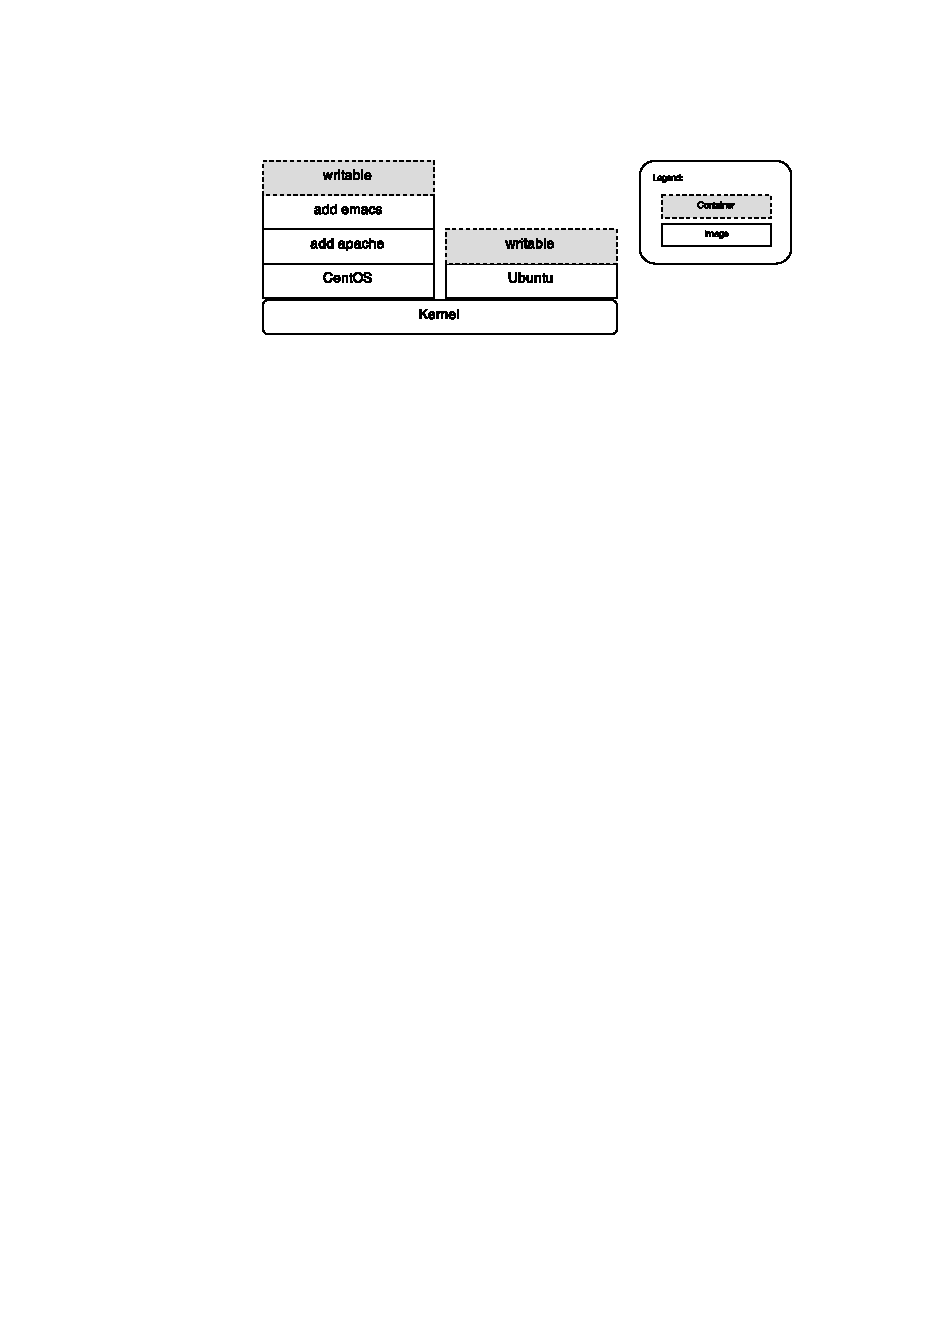
\includegraphics[width=1.0\textwidth]{cvimage.pdf}
    \caption{A graphic providing examples of the difference between containers and images in the Docker Engine. Containers are the top-most writable layers of the filesystem and represented by the rectangles with dashed lines and grey background. Images are the read-only layers used for inheritance and are represented by the rectangles with the solide lines and white background.}
\label{ch2:imagevcontainers}
\end{figure}

\section{Use Cases}\label{ch2:usecase}
\subsection{Cloud}
This is the primary target for which VM2Docker is geared. As an alternative to hosting virtual machines in the cloud, many cloud providers now offer the option to either directly use containers, run containers within a container-optimized VM, or both.

\subsection{DevOps}
Another essential audience for the Docker framework is the DevOps paradigm. DevOps is the process by which a piece of software is developed and subsequently deployed, along with the continuous revision process of simultaneous development and deployment. Historically, DevOps has been challenging to get right because of all of the dependencies a certain piece of software might have. During deployment, the software installed on a given developer's host must also be installed on the host running the deployed application. Docker provides a streamlined way to guarantee that a piece of software running on one host will run exactly the same on another host, as long as each host has the Docker Engine installed. This guarantee is an invaluable asset and is touted as the "first true" DevOps tool \cite{devops}. Ops managers may choose to deploy the Docker containers in the cloud or in their own private cluster of Docker-supported machines.

%\subsection{Benefits \& Drawbacks}\label{ch2:bd}
%https://news.ycombinator.com/item?id=8167928

\section{Industry Hype}\label{ch2:industry}

The hype over Docker, both in the open-source community as well as in the industry, has been unprecedented. In the past year and even more recently in the past six months, a number of influential players in the cloud hosting industry have begun to offer native support for running Docker containers. Specifically, Amazon has launched its own EC2 container service \cite{aws} and Google has their own container engine powered by the open-source cluster manager Kubernetes, Additionally, VMware, initially perceived to be threatened by container technology, has announced a partnership with Docker which attempts improve the overall user experience \cite{vmware}. In addition to the established cloud providers, other providers such as Tutum and Orchard, which was acquired by Docker, have been created that focus specifically on container deployment in the cloud. The excitement and popularity of the Docker framework across the industry is a testament to its utility and novelty as compared to the prior industry standard, virtual machines.

\subsection{Comparison to Virtual Machines}
While it remains to be seen whether Docker poses an immediate threat to the virtual machine landscape, it is evident that virtual machines and containers are distinct products that aren't necessarily direct competitors. Each caters to a slightly different audience.

Since Docker shares the kernel with the host, it only supports Linux-based containers and immediately discards support for legacy enterprise software that might need a Windows environment to run.

Central to the distinction between container and virtual machine is the tradeoff between density and isolation. Virtual machines offer the strongest form of isolation, comparable to that offered by physically separated hosts. Containers, on the other hand, share the kernel with the host, and therefore provide a much larger attack surface through which an attacker might be able to compromise another container on the same host. 

By giving up isolation, unlike virtual machines which incur a performance overhead, containers achieve near native performance as compared to running directly on the host itself \cite{performance}. Furthermore, the density of containers on a given host can be much higher than that of VMs. 

\begin{figure}[h]
\centering
\subfigure[Docker Container]{%
  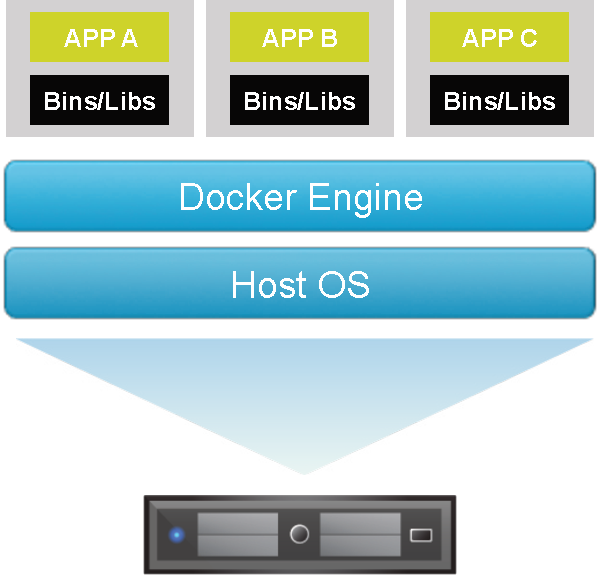
\includegraphics[width=.4\linewidth]{docker_h.pdf}
  \label{fig:sub1}}
\quad
\quad
\subfigure[Virtual Machine]{%
  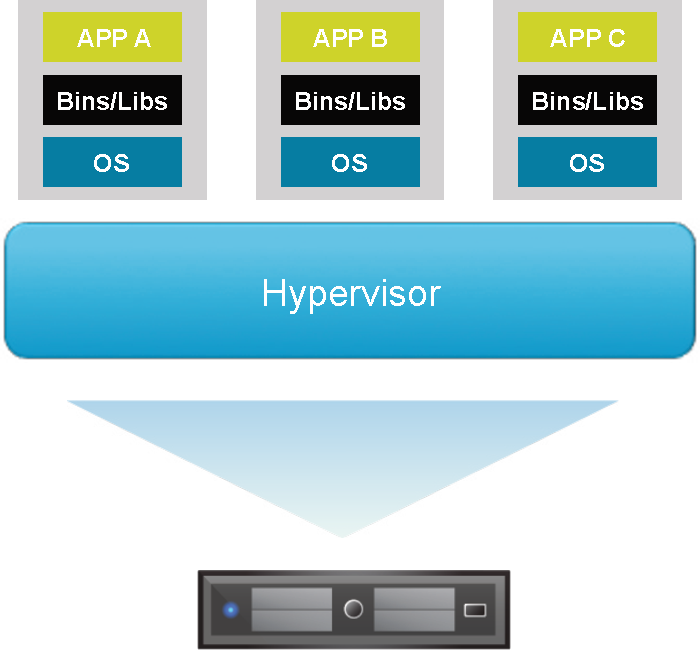
\includegraphics[width=.4\linewidth]{vm_h.pdf}
  \label{fig:sub2}}
\caption{A comparison of the components and isolation of virtual machines as compared to Docker containers. Each container consists of only an application and its dependencies and shares the underlying kernel with the host OS.}
\label{fig:test}
\end{figure}

Since Docker can run directly inside of a virtual machine, but not vice versa, there are interesting ways in which Docker and VMware VMs might be able to work together in the future to offer a streamlined experience that captures the benefits of each. Multiple, trusted, containers running in the same VM, for example, could provide stronger isolation while still achieving the portability and deployment benefits that Docker containers provide.

Another distinct advantage of VMs is there ability to perform live migrations from one host to another. VMware dubs this process vMotion\cite{vmotion}, and it is used as a direct building block for VMware's Dynamic Resource Scheduling (DRS)\cite{DRS}. Docker containers, unless running in a VM (and migrated with vMotion), cannot be live migrated to another host and instead must be shut down, moved, and started back up. CRIU\cite{CRIU} is a project under heavy active active development that attempts to bring this live migration to the container ecosystem by implementing checkpoint/restore functionality for Linux in userspace. Once completed, CRIU might be used as a primitive for dynamic resource scheduling among different Docker host. However, as of this writing, no such feature exists.
\subsection{Competitors}
Docker is one of the most successful and popular frameworks for container technology. However, there are also a number of other alternatives that are also built on top of Linux containers. 

\subsubsection{Flockport}
Flockport is a young alternative to Docker that focuses on entire virtualization workloads, instead of app delivery. As a result, Flockport does not boast the same kind of layered filesystem as Docker and instead is built on top of the LXC protocol \cite{flockport}.

\subsubsection{Spoonium}
Spoonium is a platform that attempts to bring container technologies to platforms not necessarily based on Linux. It touts many of the features of the Docker framework. Interestingly, Docker, too, has announced its intention of bringing Docker support to the Windows platform. Thus, it remains to be seen of Spoonium will experience the same kind of success that Docker has.

\subsubsection{Rocket - CoreOS}
Rocket, by CoreOS, is an alternative to Docker under heavy active development. CoreOS initially provided complete support for Docker, and their operating system was specifically built as a bare-bones operating system with the minimal amount of software installed to run Docker. A variety of disputes over the overall product vision has inspired CoreOS to develop their own take on containers, called Rocket, and we will see what sort of improvements and following this gets in the coming months and the software matures \cite{rocket}.

\subsubsection{Ubuntu - LXD}
One final player in the container field is Ubuntu and their announcement of LXD. LXD aims to build on top of LXC and serve as a hypervisor for containers. A main feature it aims to support is the live snapshotting of containers through CRIU\cite{CRIU}, which also enables them to support live migration of containers between hosts. These features are invaluable and would serve as an essential addition to the container framework, thereby bringing some of this container technology inline with that offered by VMware and vMotion and DRS \cite{vmotion,DRS}. Since LXD will work on a slightly lower level of the stack than Docker, it is possible it will also serve as an enhancement, rather than a direct competitor, to Docker \cite{lxd}.

%\subsection{Orchestration}





\appendix
\chapter{Tables}

\begin{table}
\caption{Armadillos}
\label{arm:table}
\begin{center}
\begin{tabular}{||l|l||}\hline
Armadillos & are \\\hline
our	   & friends \\\hline
\end{tabular}
\end{center}
\end{table}

\clearpage
\newpage

\chapter{Figures}

\vspace*{-3in}

\begin{figure}
\vspace{2.4in}
\caption{Armadillo slaying lawyer.}
\label{arm:fig1}
\end{figure}
\clearpage
\newpage

\begin{figure}
\vspace{2.4in}
\caption{Armadillo eradicating national debt.}
\label{arm:fig2}
\end{figure}
\clearpage
\newpage

%% This defines the bibliography file (main.bib) and the bibliography style.
%% If you want to create a bibliography file by hand, change the contents of
%% this file to a `thebibliography' environment.  For more information 
%% see section 4.3 of the LaTeX manual.

\begin{thebibliography}{99}
\begin{singlespace}
\raggedright

\bibitem{windows-docker}
``Docker CTO: Why Microsoft's Docker plans for Windows will matter to you," October 28, 2014. Available: \url{http://www.zdnet.com/docker-cto-why-microsofts-docker-plans-for-windows-will-matter-to-you-7000035150/}

\bibitem{lxc}
``PaaS under the hood, episode 1: kernel namespaces," November 28, 2012. Available: \url{http://blog.dotcloud.com/under-the-hood-Linux-kernels-on-dotcloud-part}

\bibitem{dockerregistry}
``Docker Hub Registry," [Online]. Available: \url{https://registry.hub.docker.com}

\bibitem{dockerregistry-github}
``Docker Registry," 2014. [Online]. Available: \url{https://github.com/docker/docker-registry}

\bibitem{performance}
M. G. Xavier, M. V. Neves, F. D. Rossi, T. C. Ferreto, T. Lange, and C. A. F. De Rose, ``Performance Evaluation of Container-based Virtualization for High Performance Computing Environments," 2013. [Online]. Available: \url{http://marceloneves.org/papers/pdp2013-containers.pdf}

\bibitem{vmotion}
``VMware vMotion: Virtual Machine Live Migration," [Online]. Available: \url{http://www.vmware.com/products/vsphere/features/vmotion}

\bibitem{DRS}
``vSphere Dynamic Resource Scheduler \& Distributed Power Management," [Online]. Available: \url{http://www.vmware.com/products/vsphere/features/drs-dpm}

\bibitem{CRIU}
``CRIU," 2014. [Online]. Available: \url{http://criu.org/}

\bibitem{baseimage}
``Creating a Base Image," 2014. [Online]. Available: \url{https://docs.docker.com/articles/baseimages/}

\bibitem{debootstrap}
``Debootstrap," [Online]. Available: \url{https://wiki.debian.org/Debootstrap}

\bibitem{fig}
``Fig | Fast, isolated development environments using Docker," 2014. [Online]. Available: \url{http://www.fig.sh}

\bibitem{kubernetes}
``Kubernetes," 2014. [Online]. Available: \url{https://github.com/GoogleCloudPlatform/kubernetes}

\bibitem{fleet}
``Launching Containers with fleet," 2014. [Online]. Available: \url{http://coreos.com/docs/launching-containers/launching/launching-containers-fleet/}

\bibitem{dockerindocker}
\url{https://blog.docker.com/2013/09/docker-can-now-run-within-docker/}

\end{singlespace}
\end{thebibliography}

\end{document}

